%----------------------------------------------------------------------------------------
%	PACKETS AND CONFIGURATION
%----------------------------------------------------------------------------------------

\documentclass{beamer}

\usepackage{title}  % Title settings for the presentation

%\usepackage{listings} % per snippet di codice devo ancora capire come si usano bene
%\usepackage{pdftexcmds}
%\usepackage{minted}   
%\usepackage[utf8]{inputenc}
%\usepackage[T1]{fontenc}
%\usepackage{pythontex}
%\usepackage{verbatim}

\usetheme{Copenhagen} % THEME

%----------------------------------------------------------------------------------------
%	DOCUMENT
%----------------------------------------------------------------------------------------

\begin{document}

% TITLE
\frame{\titlepage}

% Table of Contents
\begin{frame}{Project}
    \tableofcontents[hideallsubsections]
\end{frame}

% Environment and Simulation ------------------------------------------------------------

\AtBeginSection[]
{
\begin{frame}{}
    \tableofcontents[currentsection]
\end{frame}
}

% ----------------------------------------

\section{Environment and Simulator}
%-----------------------------------------
\subsection{Overview}

\begin{frame}{Fully justified}

\frametitle{Environment and Simulator}
\framesubtitle{Environment}

The environment is modelled to give as output a class cointaing all the sample values for a day of interaction for each users class.
Single arguments of the class can be specified, if desired, also to test the algorithms in limits case.

\end{frame}

% ----------------------------------------

\subsection{Randomness in the Environment}

\begin {frame} {Fully justified}

\frametitle{Environment and Simulator}
\framesubtitle{Randomness in the Environment}

To be consistent with the project and more importantly having a real scenario all the parameters, not known a priori, are randomnly generated.
For instance each day we stochastically get:

\vspace{0.5cm}
\begin{list}{-}{\setlength{\itemsep}{0.3cm}}
    \item potential clients entering the website
    \item ...
\end{list}
\vspace{0.5cm}

All these parameters are obtanied by passing through a random numer generator.

 % TODO: not sure on what the rng parameter goes to influence, to check

\end {frame}

% ----------------------------------------

\begin{frame}{Fully justified}

\frametitle{Environment and Simulator}
\framesubtitle{Randomness in the Environment}

As a part of comparing the different learners and algorithms, we had to consider the randomness in the environment.
Even though there might be determinism since the random number generator is always generating the same values across different iterations but is not determistic across all parameters.
%not sure: if i understood it corretly, if it's clear in these words

\end {frame}

% ----------------------------------------

\subsection{Parameters choise}

\begin{frame}{Fully justified}

\frametitle{Environment and Simulator}
\framesubtitle{Environment}

To sum up through the environment we can set values that define univocally:
\vspace{0.3cm}
\begin{list}{-}{\setlength{\itemsep}{0.4cm}}
    \item Users'class and their Interaction with the website.
    \item The total amount of budget to subdivide.
    \item The ratios in which every class appears in the population.
    \item The prices of each product.
    \item The budget the competitor spends in advertising
\end{list}

\end {frame}
% ----------------------------------------

\begin {frame}{Fully justified}

\frametitle{Environment and Simulator}
\framesubtitle{Users class}

In particular each Users class is modelled with:\textbf{ reservation price, steepness, shift and upper bound}
for each product, including the one of the not strategic competitor.
Since the $alpha$-functions we had choosen belong to the sigmoidal class we need these additional parameters.

\begin{figure}[⟨r⟩]  
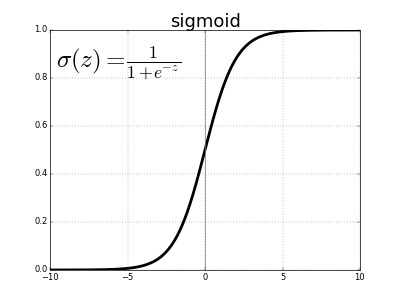
\includegraphics[height=3.8cm]{img/Graphs/sigmoid.png}
    \end{figure}
\end {frame}
%do we want to explain why we choose sigmoid here or talking? and do we want to give a realistic turn on feature and so?

% ----------------------------------------

\begin{frame}{Fully justified}

    \frametitle{Environment and Simulator}
    \framesubtitle{Example of Environment}

We see here an example of data     
    %\begin{verbatim}
 %   try try
      %  \end{verbatim}
      \begin{figure}[⟨t⟩]  
        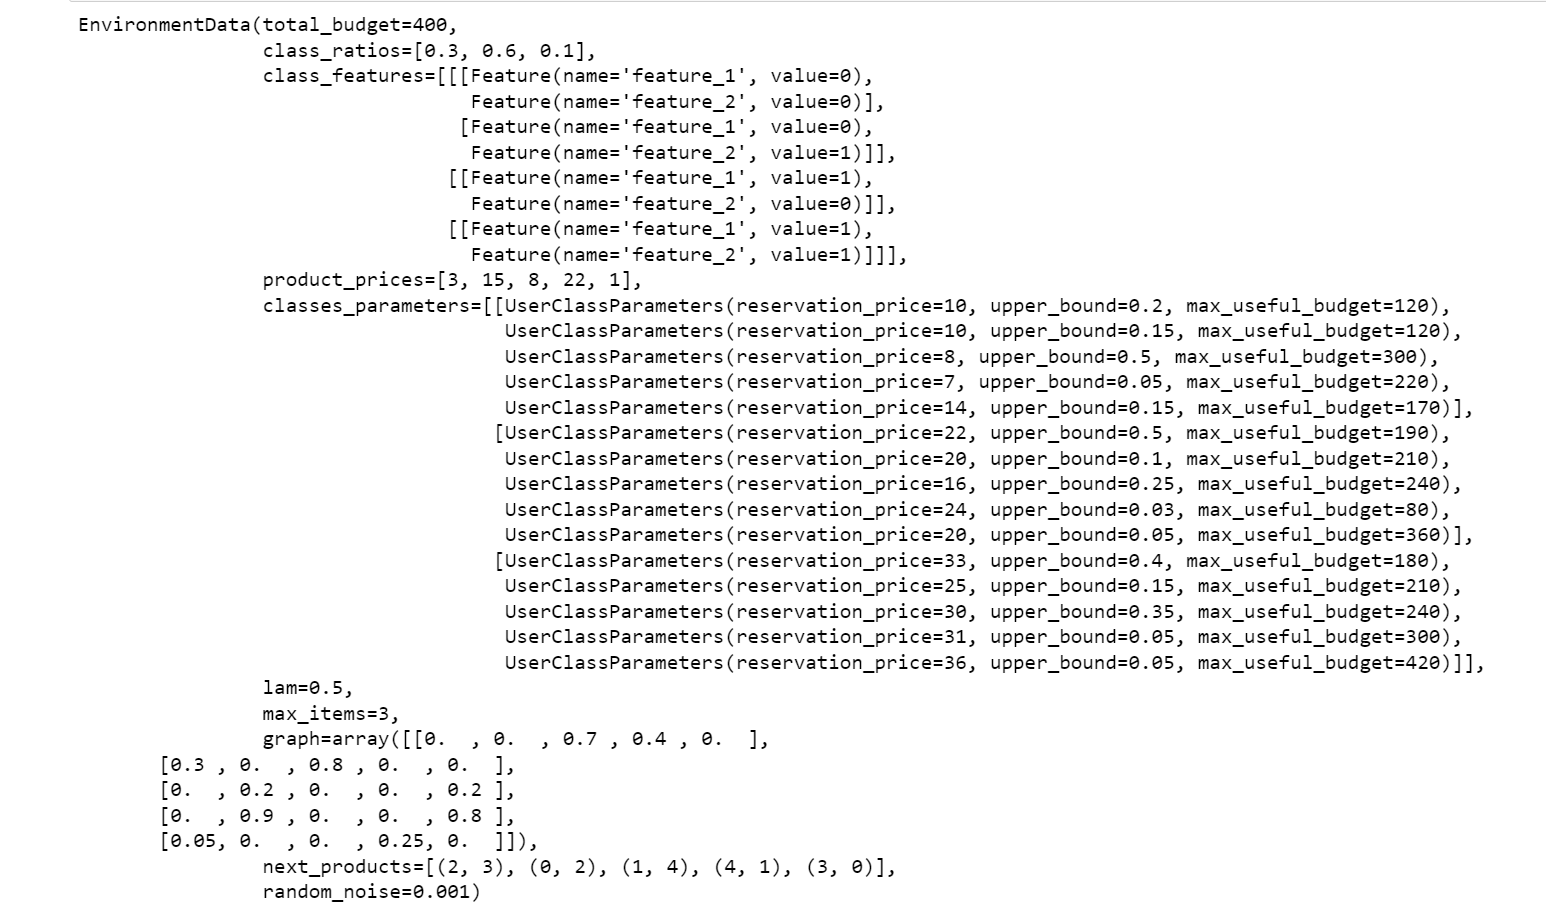
\includegraphics[height=6cm]{img/Graphs/Example_environment.png}
            \end{figure}
        %come posso aumentare leggibilità? 

\end {frame}

% ----------------------------------------

\subsection{Simulation}

\begin {frame}{Fully justified}

\frametitle{Environment and Simulator}
\framesubtitle{Daily Simulation}

Interacting with the environment we compute all the interactions of each different classes of users made each day with the website.
Repeting this simulation for each step of the time horrizon needed grants us with all the data needed to start our optimization problem.

\end{frame}

% ----------------------------------------

\begin {frame} {Fully justified}

\frametitle{Environment and Simulator}
\framesubtitle{Daily Simulation}

Here we have an instance of the interaction with the Environment.

%TODO insert either snippet of code or imagine with example of environment

%\begin{verbatim}
%get_day_of_interactions(rng,10,[90,100,120,30],env,de_noise=1e3, deterministic=False,) 
 % [Interaction(user_features=[Feature(name='feature_1', value=1), Feature(name='feature_2', value=0)], user_class=1, items_bought=array([0, 0, 1, 0, 0]), landed_on=2, edges=[]),
% Interaction(user_features=[Feature(name='feature_1', value=1), Feature(name='feature_2', value=0)], user_class=1, items_bought=array([2, 0, 1, 0, 0]), landed_on=0, edges=[(0, 2)]),
 %Interaction(user_features=[Feature(name='feature_1', value=0), Feature(name='feature_2', value=0)], user_class=0, items_bought=array([0, 0, 2, 0, 0]), landed_on=2, edges=[])]
%\end{verbatim}

\end {frame}

% ----------------------------------------

%QUESTION DO WE WANT SLIDE ON GRAPHS GENERATION OR WE can talk about it with the imagine above?

% ----------------------------------------

\subsection{"passing data to learnes"} %all subsection to write better just general idea of it.

\begin {frame}{Fully justified}

\frametitle{Environment and Simulator}
\framesubtitle{Masked Environment}

In order to be consistent and not generating uncertainty from the random number generator instead of 
comparing all the different learners on different sets of days with the same time lenght we generate 
data only once then pass only the data needed to each different learner.


\end{frame}

% ----------------------------------------

\begin {frame}{Fully justified}

\frametitle{Environment and Simulator}
\framesubtitle{Masked Environment}

This "masked" environment allows us to test the different algorithms according to the data given 
at each point and it allows us to fed the clayrvoiant alghoritm with the same set of data, 
but not masked, for a real comparison of the performance of the different algorithms.

\end{frame}

% ----------------------------------------

\begin {frame}{Fully justified}

\frametitle{Final note}
\framesubtitle{Enviroment}

%talking about deterministic flag possibility and how affect the interactions (1 slide max)

\end{frame}


% Optimization Algorithm ----------------------------------------------------------------

\AtBeginSection[]
{
\begin{frame}{}
    \tableofcontents[currentsection]
\end{frame}
}

% ----------------------------------------
\section{Optimization Algorithm}

\subsection{General Problem}

\begin{frame}{Fully justified}

\frametitle{Optimization Algorithm}
\framesubtitle{Problem Formulation}
Our aim is finding the optimal budget per campaign in order to maximize the profit.
which is defined as the difference between the expected margin and the spent in advertising
Basically, it is a maximisation subject to the obvious constraint: the sum of the daily budget can't be greater then the overall budget.

The optimization problem can be expressed as follows:
\begin{displaymath}
F=\max_{\substack{x_i\in B}} \sum_{i=0}^n \alpha_i(x_i)p_i-x_i \ s.t. \sum_{i=0}^n x_i\leq B
\end{displaymath}

\end{frame}

% ----------------------------------------

\subsection{Algorithm}


\begin {frame} {Fully justified}

\frametitle{}
\framesubtitle{}
%talking about the code in words

\end {frame}

% ----------------------------------------

\begin {frame} {Fully justified}

\frametitle{Algorithm Optimization}
\framesubtitle{}
%add snippet of code  

\end {frame}

% ----------------------------------------


% Uncertain alpha functions -------------------------------------------------------------

\AtBeginSection[]
{
\begin{frame}{}
    \tableofcontents[currentsection]
\end{frame}
}

% ----------------------------------------

\section{Uncertain alpha-functions}

\begin {frame}{Fully justified}

\frametitle{Uncertain alpha-functions}
Since the feature of the users are \textbf{not osservable}, the algorithm take as input the aggregated list of interactions.
It tries to estimate the aggregated $alpha$-function and the reward of each single product

\end{frame}

% ----------------------------------------

\begin {frame}{Fully justified}

\frametitle{Uncertain $alpha$-functions}
\framesubtitle{Result}
% TODO: going to insert some graph of clayrvoiantv stupid v ts v ucb1

\end{frame}

% Uncertain alpha functions and number of items sold ------------------------------------

%\section{Uncertain $alpha$-functions and number of items sold}

% Uncertain graph weights ---------------------------------------------------------------

%\section{Uncertain Graph Weights}

% Non-stationary demand curve -----------------------------------------------------------

%\section{Non-stationary demand curve}

% Context generation --------------------------------------------------------------------

%\section{Context generation}

\end{document}


%NOTE TO THE US:
%%\centering if we want the presentation to be power-point style 